\documentclass[10pt,a4paper]{article}
\usepackage[utf8]{inputenc}
\usepackage[T1]{fontenc}
\usepackage[english,spanish]{babel}
\usepackage{indentfirst}
\usepackage{anysize}
\marginsize{2,5cm}{1,8cm}{1.5cm}{1,7cm}
\usepackage[psamsfonts]{amssymb}
\usepackage{amssymb}
\usepackage{amsfonts}
\usepackage{amsmath}
\usepackage{amsthm}
\usepackage{multicol}
\usepackage{multirow}
\usepackage{graphicx}
\usepackage[hidelinks]{hyperref}
\usepackage{caption}
\usepackage{subcaption}
\usepackage{tocloft}
\usepackage{booktabs}
\usepackage{listings}
\usepackage{xcolor}
\usepackage{float}
\usepackage{tikz}
\usetikzlibrary{positioning, arrows.meta}
\renewcommand{\cftsecleader}{\cftdotfill{\cftdotsep}}
\setlength{\cftbeforesecskip}{5pt}
\setlength{\cftbeforesubsecskip}{1pt}
\addto\captionsspanish{\renewcommand*\contentsname{Contenido}}
\renewcommand{\thepage}{}
\theoremstyle{definition}
\renewcommand{\thefootnote}{\fnsymbol{footnote}}

\lstset{
  basicstyle=\ttfamily\scriptsize,
  breaklines=true,
  frame=single,
  columns=fullflexible,
  keepspaces=true,
  showstringspaces=false,
  commentstyle=\color{gray},
  numbers=none
}

\begin{document}

\title{Resultados de las operaciones policiales a nivel nacional: an\'alisis con Spark, Scala y PostgreSQL}
\date{}
\maketitle

\begin{center}
	Integrantes:\\
	\vspace{5pt}
	{\large Luis Antonio Rojas Huaroc}\\
	e-mail: larojash@uni.pe\\
	\vspace{5pt}
	{\large Breiner Catalino Morales}\\
	e-mail: breiner.catalino.m@uni.pe\\
	\vspace{5pt}
	Universidad Nacional de Ingenier\'ia, Facultad de Ciencias
\end{center}
\vspace{5pt}
\begin{center}
	Curso:\\
	\vspace{5pt}
	{\large CC531 A -- An\'alisis en Macrodatos 2026-2}\\
	{\large Laboratorio 03}\\
\end{center}
\vspace{20pt}

\begin{abstract}
{\small
\hspace*{0.5cm}
Se configur\'o un entorno Apache Spark 3.3.2 (con Hadoop 3.3.0) y Scala 2.12.15 sobre Windows, junto
con PostgreSQL 15.13, para analizar el dataset \emph{Resultados de las operaciones policiales a nivel
nacional} del Ministerio del Interior (MININTER/CENOPPOL), categor\'ia Seguridad y Justicia de la
Plataforma Nacional de Datos Abiertos, con 30\,456 registros de los a\~nos 2023 a 2025. Se resolvieron
cinco consultas en Scala sobre RDD usando MapReduce puro (agrupamiento con m\'aximos/m\'inimos,
estad\'isticos de un campo decimal, y tres consultas con MapReduce triple), se dise\~n\'o un esquema en
estrella en PostgreSQL (dos dimensiones y una tabla de hechos) poblado mediante un proceso ETL completo
en Spark, y se resolvieron adem\'as 18 consultas con la API de DataFrame de Spark SQL (\texttt{groupBy},
\texttt{filter}, los cuatro tipos de \texttt{join}, funciones de
\texttt{org.apache.spark.sql.functions.\_}) y con vistas temporales y SQL puro, exportando parte de los
resultados a Excel con Spark. Todas las consultas se verificaron cruzando resultados entre s\'i (por
ejemplo, el mayor valor hist\'orico de dinero incautado coincide exactamente entre la consulta de
m\'aximos/m\'inimos y la de estad\'isticos).\\

\textbf{Palabras clave:} Apache Spark, Scala, MapReduce, Spark SQL, PostgreSQL, ETL, seguridad
ciudadana.
}
\end{abstract}

\pagenumbering{arabic}

\tableofcontents

\vspace{20pt}
\hrule
\vspace{10pt}

\section{Introducci\'on}

Este informe corresponde al Laboratorio 03 del curso \emph{An\'alisis en Macrodatos}. El trabajo exige
configurar Apache Spark y Spark SQL, elegir un conjunto de datos de la Plataforma Nacional de Datos
Abiertos (PNDA) en la categor\'ia \textbf{Seguridad y Justicia} --distinto al usado por cualquier otro
grupo del curso--, resolver consultas en Scala sobre RDD usando MapReduce puro, almacenar el dataset en
una base de datos PostgreSQL con una arquitectura de tablas dise\~nada por el propio equipo, resolver
consultas adicionales con la API de DataFrame de Spark SQL y con vistas temporales, y exportar parte de
los resultados a Excel.

\subsection{Selecci\'on del dataset}
La primera opci\'on considerada, \emph{Denuncias policiales registradas a nivel nacional [MININTER]},
se descart\'o al verificar que ya estaba siendo usada por otro grupo del curso. En su lugar se eligi\'o
\textbf{Resultados de las operaciones policiales a nivel nacional [MININTER]}, publicado por el
Observatorio Nacional de Seguridad Ciudadana con datos de la Central de Operaciones Policiales
(CENOPPOL), disponible en
\url{https://www.datosabiertos.gob.pe/dataset/resultados-de-las-operaciones-policiales-nivel-nacional-mininter}.
Se descargaron los tres recursos CSV correspondientes a los a\~nos 2023, 2024 y 2025 y se combinaron en
un \'unico archivo de \textbf{30\,456 registros}.

\section{Datos}

\subsection{Fuente}
\begin{itemize}
  \item \textbf{T\'itulo:} Resultados de las operaciones policiales a nivel nacional [MININTER].
  \item \textbf{Instituci\'on:} Ministerio del Interior (MININTER), Observatorio Nacional de Seguridad
    Ciudadana, con datos de la Central de Operaciones Policiales (CENOPPOL) de la Polic\'ia Nacional del
    Per\'u.
  \item \textbf{Plataforma:} Plataforma Nacional de Datos Abiertos (PNDA, \url{https://www.datosabiertos.gob.pe}).
  \item \textbf{Categor\'ia PNDA:} Seguridad y Justicia.
  \item \textbf{Frecuencia de actualizaci\'on:} mensual.
  \item \textbf{Licencia:} Open Data Commons Attribution License (ODC-BY).
  \item \textbf{Archivos usados:} \texttt{DATASET\_Produccion Policial\_2023.csv},
    \texttt{..\_2024.csv}, \texttt{..\_2025.csv}.
\end{itemize}

\subsection{Rubro y teor\'ia detr\'as de los datos}
El dataset pertenece al \'ambito de \textbf{seguridad ciudadana y orden p\'ublico}: registra, mes a mes
y por dependencia policial, el resultado cuantificado de las operaciones de la PNP contra la
criminalidad organizada, el narcotr\'afico, el contrabando y las infracciones de tr\'ansito. Cada fila
es un \emph{evento de producci\'on policial}: una dependencia, en un mes y a\~no dados, report\'o cierta
cantidad de un tipo de resultado (armas incautadas, kilos de droga decomisados, dinero incautado,
detenidos, etc.). Es, en esencia, un registro administrativo de desempe\~no operativo: la teor\'ia detr\'as
es que la frecuencia e intensidad de estos resultados refleja tanto la actividad delictiva de una zona
como la capacidad de respuesta policial asignada a ella, dos variables que no se pueden separar solo con
estos datos (un n\'umero alto de incautaciones puede significar m\'as delito o m\'as operativos, no
necesariamente ambos).

\subsection{Descripci\'on y caracter\'isticas}
El archivo combinado tiene 30\,456 filas y 6 columnas:
\begin{itemize}
  \item \texttt{A\~NO} (2023-2025), \texttt{MES} (abreviatura de 3 letras en espa\~nol).
  \item \texttt{VARIABLE}: 18 valores distintos, el tipo de resultado operativo (ver Cuadro~\ref{tab:variables}).
  \item \texttt{DEPENDENCIAS}: 53 unidades policiales distintas en el periodo combinado (jefaturas
    regionales ``RP'', frentes policiales ``FP'', direcciones especializadas como DIRANDRO, DIRILA,
    DIVIAC, etc.).
  \item \texttt{DIR\_REG\_FRE}: clasificaci\'on de la dependencia en \texttt{Regi\'on}, \texttt{Frente},
    \texttt{DIRNIC} (Direcci\'on contra el Crimen Organizado) o \texttt{DIRNOS} (Direcciones Operativas
    Especializadas).
  \item \texttt{VALOR}: campo num\'erico decimal (hasta 3 decimales), la cantidad reportada. Incluye
    conteos enteros (personas, unidades) y magnitudes continuas reales (kilos de droga con hasta 3
    decimales, soles incautados con 2 decimales).
\end{itemize}

\begin{table}[H]
\centering\small
\begin{tabular}{@{}llr@{}}
\toprule
\textbf{Categor\'ia derivada} & \textbf{Unidad} & \textbf{Variables originales (de 18)}\\
\midrule
Droga & Kilos / Envoltorios & PBC, Marihuana, CC (clorhidrato de coca\'ina) -- 6\\
Dinero & Soles & DINERO INCAUTADO (SOLES) -- 1\\
Contrabando & Soles & CONTRABANDO (VALORIZACION) -- 1\\
Arma & Unidades & Armas blancas, armas de fuego -- 2\\
Detenido & Personas & Diversos delitos (peruanos/extranjeros), requisitoriados -- 3\\
Organizaci\'on criminal & Unidades & Bandas y organizaciones desarticuladas -- 2\\
Migraci\'on & Personas & Intervenci\'on extranjeros (ley migratoria) -- 1\\
Operativo & Unidades & OPERATIVOS -- 1\\
Infracci\'on de tr\'ansito & Unidades & Papeletas RNT -- 1\\
\bottomrule
\end{tabular}
\caption{Las 18 variables originales del dataset, agrupadas en 9 categor\'ias derivadas (usadas en la
base de datos y en las consultas de Spark SQL).}
\label{tab:variables}
\end{table}

\subsection{Preprocesamiento y limitaciones}
\begin{itemize}
  \item El n\'umero de dependencias distintas en el periodo combinado (53) es mayor al de un a\~no
    individual (46 en 2024 solo), porque algunas dependencias aparecen \'unicamente en 2023 o 2025.
  \item \textbf{Problema de calidad de datos encontrado:} 432 filas de 2025 (1.4\,\% del total) traen
    \texttt{DIR\_REG\_FRE} mal copiado --repite el nombre de la dependencia (\texttt{RP ICA} /
    \texttt{RP TUMBES}) en vez de \texttt{Regi\'on}--. Se corrigi\'o en el proceso ETL (secci\'on
    \ref{sec:etl}) y tambi\'en en las consultas de MapReduce que usan esta columna directamente sobre el
    CSV.
  \item No hay valores nulos ni filas mal formadas (verificado: las 30\,456 filas tienen exactamente 6
    campos separados por coma).
\end{itemize}

\section{Entorno y metodolog\'ia}
Se instal\'o, sin usar ning\'un instalador que requiriera privilegios de administrador:
\begin{itemize}
  \item \textbf{Apache Spark 3.3.2} (con Hadoop 3.3.0), \textbf{Scala 2.12.15}, Java 8 -- mismas
    versiones usadas en clase (\texttt{instalacion spark3.3.2.pdf}).
  \item \textbf{PostgreSQL 15.13} (binarios port\'atiles, sin servicio de Windows) y el controlador JDBC
    \texttt{postgresql-42.7.6.jar} -- mismas versiones de \texttt{Semana 11/instalacion.txt}.
\end{itemize}
Todas las consultas de Scala se ejecutan con \texttt{spark-shell}, cargando el controlador JDBC con
\texttt{--driver-class-path} / \texttt{--jars} cuando se necesita conexi\'on a PostgreSQL, siguiendo el
patr\'on visto en clase (\texttt{Semana 11/db.scala}).

\section{Resultados: Scala + Spark con MapReduce (RDD)}

\subsection{3.a -- Mayor y menor valor por tipo de resultado (MapReduce)}
\textbf{Tipo:} MapReduce simple (\texttt{map} + \texttt{reduceByKey}). \textbf{Pregunta:} ¿cu\'al es el
mayor y el menor valor registrado hist\'oricamente (2023-2025) para cada uno de los 18 tipos de
resultado operativo?

\textbf{Soluci\'on.} Se mapea cada registro a (\texttt{VARIABLE}, \texttt{VALOR}) y se aplican dos
\texttt{reduceByKey} independientes, uno con \texttt{math.max} y otro con \texttt{math.min}.
\begin{lstlisting}
val pares = datos.map(_.split(",")).map(c => (c(2), c(5).toDouble))
val maxPorTipo = pares.reduceByKey((a, b) => math.max(a, b))
val minPorTipo = pares.reduceByKey((a, b) => math.min(a, b))
\end{lstlisting}

\textbf{Salida (extracto):} el m\'inimo es 0 en los 18 tipos (hay meses sin incidencia). Los m\'aximos
m\'as relevantes: \texttt{CONTRABANDO (VALORIZACION)} S/\,513\,820\,390; \texttt{DINERO INCAUTADO
(SOLES)} S/\,4\,028\,271.78; \texttt{MARIHUANA (KILOS)} 29\,924.75\,kg; \texttt{PBC (KILOS)}
13\,717.359\,kg; \texttt{PAPELETAS INFRACCION RNT} 91\,263; \texttt{OPERATIVOS} 21\,884.

\begin{figure}[H]
\centering
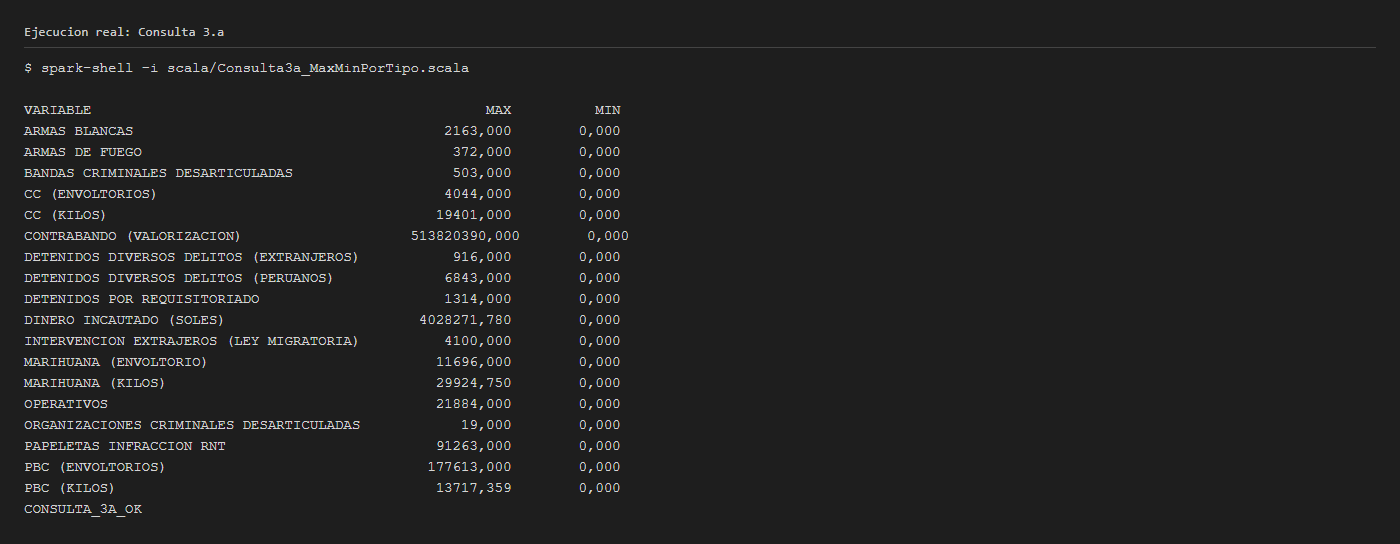
\includegraphics[width=0.95\linewidth]{capturas/img_3a.png}
\caption{Ejecuci\'on real de la consulta 3.a en \texttt{spark-shell}.}
\end{figure}

\textbf{Interpretaci\'on.} El valor m\'aximo de \texttt{DINERO INCAUTADO (SOLES)} (S/\,4\,028\,271.78)
coincide exactamente con el mayor de la consulta 3.b, lo que confirma que ambas consultas, programadas e
independientemente, miden lo mismo sobre el mismo campo.

\subsection{3.b -- Estad\'isticos del dinero incautado (MapReduce)}
\textbf{Tipo:} MapReduce con acumulador compuesto (\texttt{aggregate}) m\'as un \texttt{sortBy} para
la mediana. \textbf{Pregunta:} ¿cu\'anto dinero en soles incauta en promedio la PNP por registro, cu\'al
es la media (mediana), cu\'an dispersos son esos montos, y cu\'ales son el mayor y el menor?

\textbf{Soluci\'on.} Se filtra \texttt{VARIABLE = "DINERO INCAUTADO (SOLES)"}. El enunciado pide
promedio y media por separado: aqu\'i el \textbf{promedio} es la media aritm\'etica y la \textbf{media}
es la mediana. Un acumulador \texttt{(suma, sumaCuadrados, conteo, m\'aximo, m\'inimo)} da promedio,
varianza (poblacional), desviaci\'on, mayor y menor; la mediana se obtiene ordenando el RDD y tomando
el promedio de los dos valores centrales ($n$ par).
\begin{lstlisting}
def combinar(a: Acum, v: Double): Acum =
  (a._1 + v, a._2 + v * v, a._3 + 1L, math.max(a._4, v), math.min(a._5, v))
val promedio = suma / n
val mediana = ordenados.filter(idx == n/2-1 || idx == n/2).values.mean()
\end{lstlisting}

\textbf{Salida:} $n=1692$ registros; promedio S/\,31\,840.98; mediana S/\,1\,799.30; desviaci\'on
est\'andar S/\,142\,260.99; mayor S/\,4\,028\,271.78; menor S/\,0.00.

\begin{figure}[H]
\centering
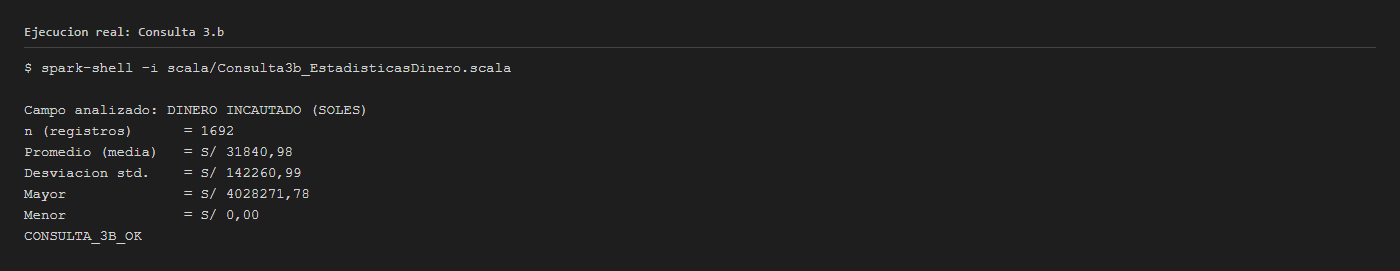
\includegraphics[width=0.85\linewidth]{capturas/img_3b.png}
\caption{Ejecuci\'on real de la consulta 3.b en \texttt{spark-shell}.}
\end{figure}

\textbf{Interpretaci\'on.} La mediana (S/\,1\,799.30) es mucho menor que el promedio
(S/\,31\,840.98), y la desviaci\'on (S/\,142\,260.99) es m\'as de 4 veces el promedio: la
distribuci\'on es muy asim\'etrica. La mayor\'ia de los registros son montos peque\~nos o cero, y unos
pocos operativos grandes (el m\'aximo de S/\,4 millones) concentran una fracci\'on desproporcionada del
total incautado.

\subsection{3.c -- Tres consultas con MapReduce triple}

\subsubsection{3.c.1 -- Desviaci\'on de OPERATIVOS por dependencia respecto al promedio nacional}
\textbf{Pregunta:} ¿qu\'e dependencias reportan muchos m\'as (o muchos menos) operativos de lo normal,
comparadas con el promedio nacional?

\textbf{Soluci\'on (3 jobs encadenados).} \emph{Job 1}: \texttt{reduceByKey} de (suma, conteo) por
dependencia. \emph{Job 2}: \texttt{reduce} de esas sumas/conteos a un \'unico promedio nacional.
\emph{Job 3}: \texttt{map} de cada dependencia a su desviaci\'on (promedio propio $-$ promedio nacional),
ordenado por valor absoluto.
\begin{lstlisting}
val porDependencia = datos.map(c => (c(3), (c(5).toDouble, 1L))).reduceByKey((a,b)=>(a._1+b._1,a._2+b._2))
val promedioNacional = sumaNacional / conteoNacional
val desviaciones = porDependencia.map{case(dep,(s,n))=>(dep, s/n, s/n-promedioNacional, n)}
\end{lstlisting}

\textbf{Salida.} Promedio nacional: 2070.90 operativos por registro ($n=1692$). Mayor desviaci\'on
positiva: \textbf{RP Lima} (promedio propio 12\,677.83, desviaci\'on $+10\,606.94$), seguida de RP Cusco
($+6080.13$), RP Ancash ($+3976.21$), RP Piura ($+3713.05$). Mayor desviaci\'on negativa: DIRFAM
(promedio 0, desviaci\'on $-2070.90$).

\begin{figure}[H]
\centering
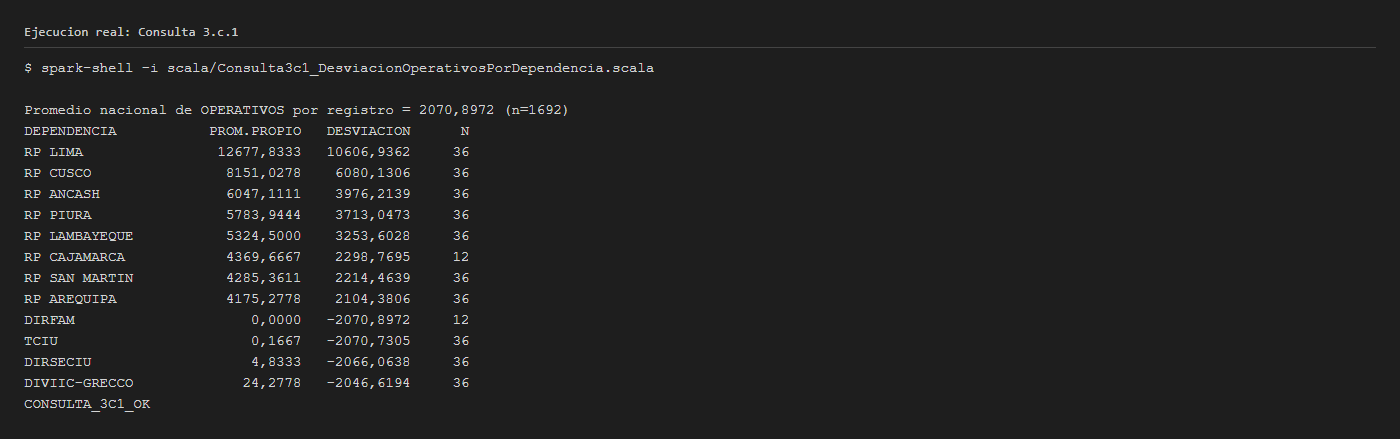
\includegraphics[width=0.85\linewidth]{capturas/img_3c1.png}
\caption{Ejecuci\'on real de la consulta 3.c.1 en \texttt{spark-shell}.}
\end{figure}

\textbf{Interpretaci\'on.} Lima concentra la mayor actividad operativa del pa\'is por ser la capital y la
regi\'on m\'as poblada; las direcciones especializadas sin funci\'on territorial directa (como DIRFAM)
no reportan ``operativos'' en este sentido, de ah\'i su desviaci\'on m\'axima negativa.

\subsubsection{3.c.2 -- Porcentaje de cada droga dentro del total de kilos por regi\'on/frente}
\textbf{Pregunta:} dentro de cada regi\'on/frente, ¿qu\'e droga (PBC, marihuana o clorhidrato de
coca\'ina) representa la mayor proporci\'on de los kilos incautados?

\textbf{Soluci\'on (3 jobs).} \emph{Job 1}: suma de kilos por (regi\'on, droga). \emph{Job 2}: reagrupa
la salida del job 1 por regi\'on y suma el total. \emph{Job 3}: calcula el porcentaje de cada droga
dentro de su regi\'on.

\textbf{Salida.}
\begin{table}[H]
\centering\small
\begin{tabular}{@{}llrr@{}}
\toprule
\textbf{Regi\'on/Frente} & \textbf{Droga predominante} & \textbf{Kilos} & \textbf{\% del total}\\
\midrule
DIRNIC & Marihuana & 141\,030.07 & 36.38\,\%\\
DIRNOS & CC (clorhidrato) & 4096.69 & 67.06\,\%\\
Frente & CC (clorhidrato) & 11\,501.08 & 83.14\,\%\\
Regi\'on & Marihuana & 91\,960.67 & 82.67\,\%\\
\bottomrule
\end{tabular}
\caption{Droga predominante por regi\'on/frente (de 3.c.2).}
\end{table}

\begin{figure}[H]
\centering
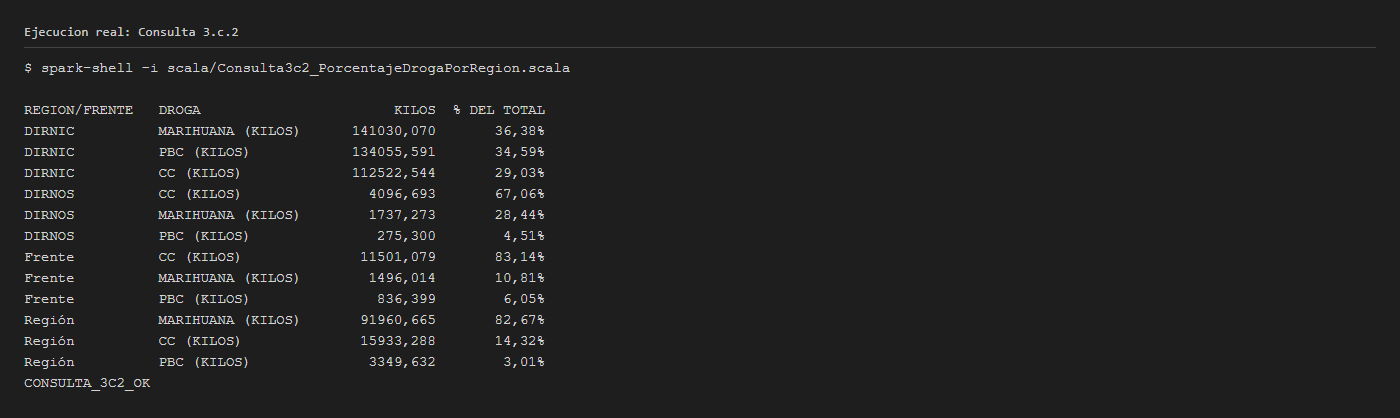
\includegraphics[width=0.85\linewidth]{capturas/img_3c2.png}
\caption{Ejecuci\'on real de la consulta 3.c.2 en \texttt{spark-shell}.}
\end{figure}

\textbf{Interpretaci\'on.} Las regiones y frentes territoriales (Regi\'on, Frente) decomisan sobre todo
marihuana y clorhidrato de coca\'ina en bruto, mientras que DIRNIC --encargada del crimen organizado a
nivel nacional-- tiene una distribuci\'on m\'as pareja entre las tres drogas, consistente con operar
contra redes de tr\'afico m\'as grandes y diversificadas.

\subsubsection{3.c.3 -- Variaci\'on interanual del dinero incautado promedio mensual}
\textbf{Pregunta:} ¿creci\'o o disminuy\'o, a\~no a a\~no, el promedio mensual de dinero incautado a
nivel nacional entre 2023 y 2025?

\textbf{Soluci\'on (3 jobs).} \emph{Job 1}: suma y conteo de \texttt{DINERO INCAUTADO} por a\~no.
\emph{Job 2}: promedio mensual por a\~no (suma del a\~no / 12). \emph{Job 3}: \% de variaci\'on respecto
al a\~no anterior.

\textbf{Salida.}
\begin{table}[H]
\centering\small
\begin{tabular}{@{}rrrr@{}}
\toprule
\textbf{A\~no} & \textbf{Suma total (S/)} & \textbf{Promedio mensual (S/)} & \textbf{\% variaci\'on}\\
\midrule
2023 & 11\,704\,529.39 & 975\,377.45 & --\\
2024 & 25\,880\,605.54 & 2\,156\,717.13 & $+121.12\%$\\
2025 & 16\,289\,794.79 & 1\,357\,482.90 & $-37.06\%$\\
\bottomrule
\end{tabular}
\caption{Promedio mensual de dinero incautado y variaci\'on interanual.}
\end{table}

\begin{figure}[H]
\centering
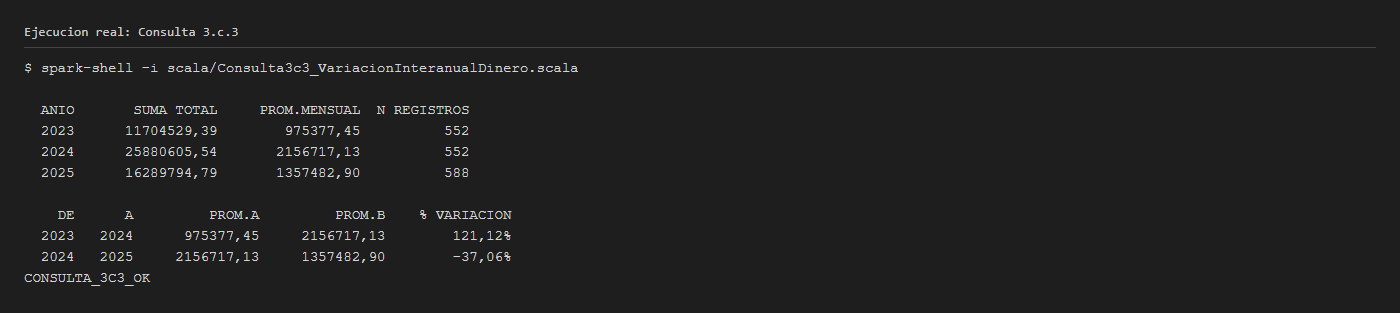
\includegraphics[width=0.75\linewidth]{capturas/img_3c3.png}
\caption{Ejecuci\'on real de la consulta 3.c.3 en \texttt{spark-shell}.}
\end{figure}

\textbf{Interpretaci\'on.} El dinero incautado promedio mensual m\'as que se duplic\'o entre 2023 y 2024
y luego cay\'o un tercio hacia 2025; sin m\'as contexto (campa\~nas espec\'ificas, cambios normativos) no
se puede atribuir la ca\'ida a un solo factor, pero el patr\'on confirma que esta variable es altamente
vol\'atil a\~no a a\~no, coherente con la alta desviaci\'on est\'andar encontrada en 3.b.

\section{Proceso ETL para la base de datos}
\label{sec:etl}

\subsection{Arquitectura de la base de datos}
Se dise\~n\'o un \textbf{esquema en estrella} con dos tablas dimensi\'on y una tabla de hechos:

\begin{figure}[H]
\centering
\begin{tikzpicture}[
  entidad/.style={draw, rectangle, rounded corners, minimum width=4.2cm, align=left, font=\small},
  titulo/.style={font=\small\bfseries}
]
\node[entidad] (dep) at (0,0) {
  \textbf{dim\_dependencia}\\
  \underline{dependencia\_id} (PK)\\
  nombre\\
  dir\_reg\_fre
};
\node[entidad] (hecho) at (5.2,0) {
  \textbf{hecho\_resultado\_operativo}\\
  \underline{id} (PK)\\
  anio, mes\\
  dependencia\_id (FK)\\
  variable\_id (FK)\\
  valor
};
\node[entidad] (var) at (10.4,0) {
  \textbf{dim\_variable}\\
  \underline{variable\_id} (PK)\\
  nombre\\
  categoria\\
  unidad
};
\draw[-{Latex[length=2mm]}] (dep.east) -- (hecho.west) node[midway, above, font=\scriptsize] {1:N};
\draw[-{Latex[length=2mm]}] (var.west) -- (hecho.east) node[midway, above, font=\scriptsize] {1:N};
\end{tikzpicture}
\caption{Diagrama Entidad-Relaci\'on: esquema en estrella con 2 dimensiones (53 y 18 filas) y 1 tabla de
hechos (30\,456 filas).}
\end{figure}

\subsection{Extract}
Se descargaron los 3 archivos CSV (2023, 2024, 2025) directamente de la PNDA y se combinaron en un solo
archivo, verificando que las 30\,456 filas tuvieran exactamente 6 campos cada una.

\subsection{Transform}
Realizado \'integramente en Spark/Scala (\texttt{ETL\_CargarDatos.scala}):
\begin{itemize}
  \item Correcci\'on de las 432 filas con \texttt{DIR\_REG\_FRE} mal copiado (ver secci\'on de
    preprocesamiento).
  \item Derivaci\'on de \texttt{categoria} y \texttt{unidad} a partir del texto de \texttt{VARIABLE},
    mediante una cadena de \texttt{when/otherwise} (Cuadro~\ref{tab:variables}).
  \item Asignaci\'on de llaves subrogadas (\texttt{dependencia\_id}, \texttt{variable\_id}) con la
    funci\'on de ventana \texttt{row\_number()} sobre el nombre, para un orden determinista.
\end{itemize}
\begin{lstlisting}
val categoriaCalc = when(categoriaExpr.contains("ARMAS"), "Arma")
  .when(categoriaExpr.rlike("^(CC|MARIHUANA|PBC)"), "Droga")
  .when(categoriaExpr.contains("DINERO"), "Dinero")
  ...otherwise("Otro")
val dimDependenciaDF = limpioDF.select("dependencia","dir_reg_fre").distinct()
  .withColumn("dependencia_id", row_number().over(Window.orderBy("dependencia")))
\end{lstlisting}

\subsection{Load}
La tabla de hechos se arma uniendo el detalle limpio con las dos dimensiones ya calculadas (para quedarse
solo con las llaves for\'aneas), y las tres tablas se escriben a PostgreSQL por JDBC
(\texttt{df.write.format("jdbc")...}), sobre las tablas creadas previamente con \texttt{CREATE TABLE}
(\texttt{db/01\_crear\_tablas.sql}).

\begin{figure}[H]
\centering
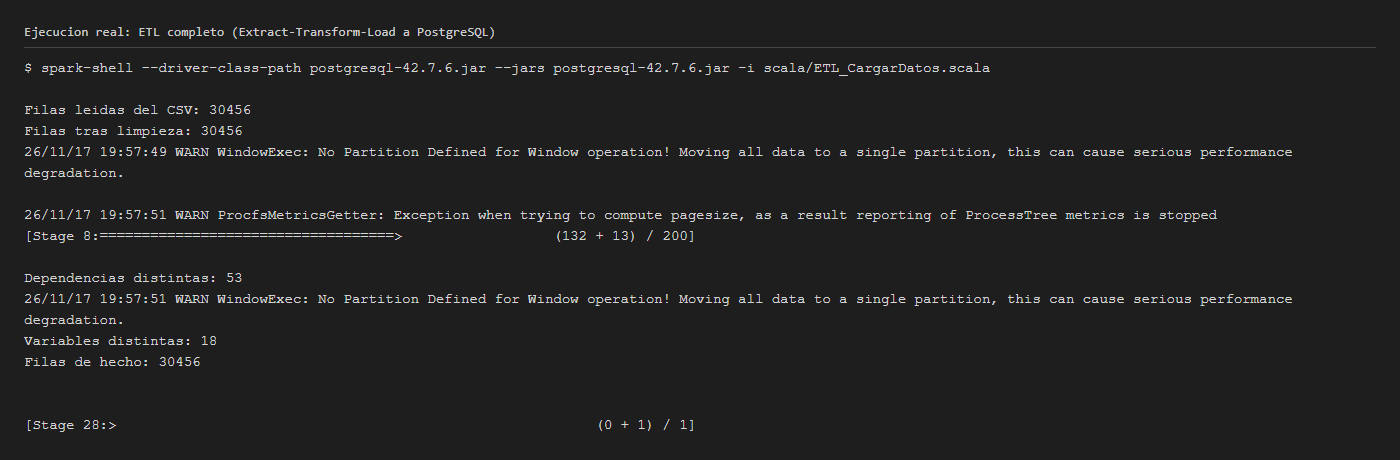
\includegraphics[width=0.95\linewidth]{capturas/img_etl.png}
\caption{Ejecuci\'on real del script de ETL completo en \texttt{spark-shell}: lectura, limpieza y carga
a las 3 tablas de PostgreSQL.}
\end{figure}

\begin{figure}[H]
\centering
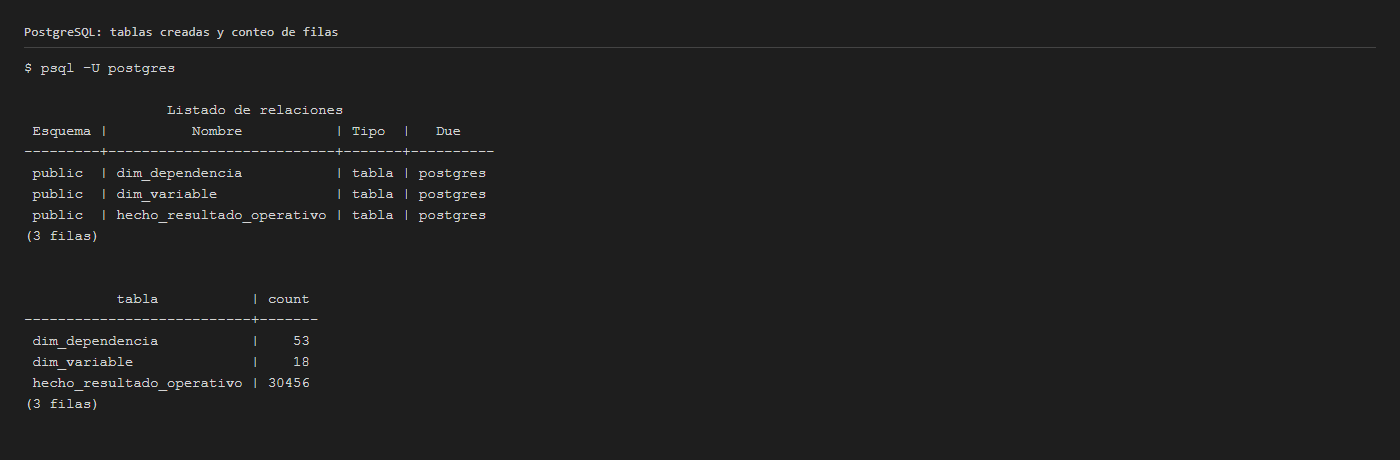
\includegraphics[width=0.85\linewidth]{capturas/db_tablas_conteo.png}
\caption{Las 3 tablas creadas en PostgreSQL y su conteo de filas tras el ETL: 53 dependencias, 18
variables, 30\,456 hechos.}
\end{figure}

\begin{figure}[H]
\centering
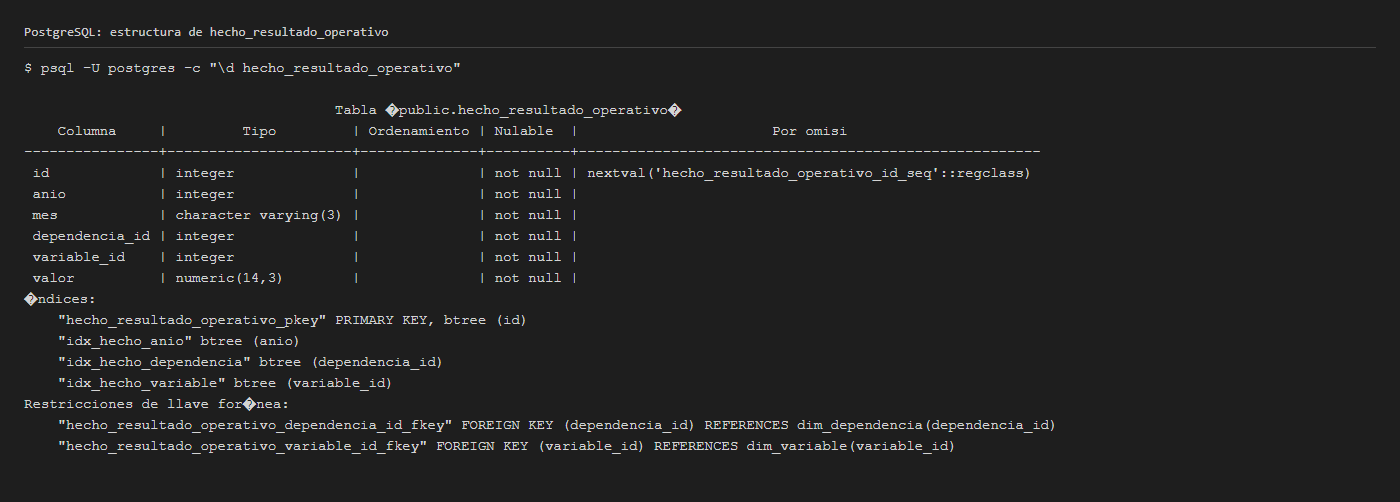
\includegraphics[width=0.9\linewidth]{capturas/db_estructura_tabla.png}
\caption{Estructura de \texttt{hecho\_resultado\_operativo}: llaves primaria y for\'aneas, \'indices.}
\end{figure}

\begin{figure}[H]
\centering
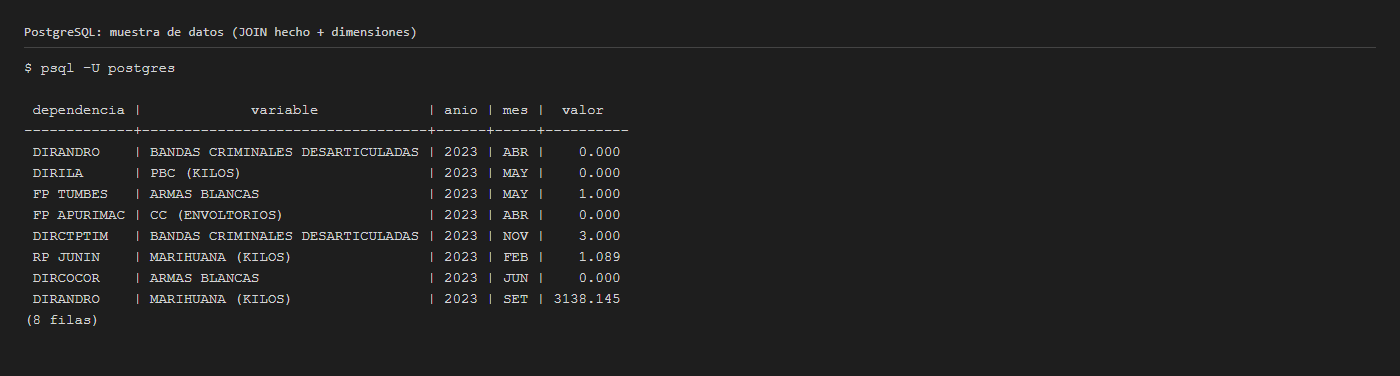
\includegraphics[width=0.85\linewidth]{capturas/db_muestra_join.png}
\caption{Muestra de datos reales obtenida con un \texttt{JOIN} entre la tabla de hechos y las dos
dimensiones.}
\end{figure}

\section{Resultados: Spark SQL con API de DataFrame}

\subsection{5.a -- Cuatro consultas con \texttt{groupBy} + \texttt{filter} (2+ columnas)}
\begin{enumerate}
  \item Suma de \texttt{valor} por (a\~no, categor\'ia), filtrando \texttt{valor > 0}. Ejemplo: en 2024,
    \texttt{Contrabando} suma S/\,838\,490\,746.64, muy por encima de las dem\'as categor\'ias ese a\~no.
  \item Conteo de registros por (dependencia, mes), filtrando \texttt{a\~no = 2024}: la mayor\'ia de
    combinaciones tiene 18 registros (uno por cada una de las 18 variables).
  \item Suma de kilos por (regi\'on/frente, categor\'ia), filtrando \texttt{unidad = 'Kilos'}: DIRNIC
    lidera con 387\,608.2\,kg, seguida de Regi\'on con 111\,243.6\,kg.
  \item Total por (a\~no, unidad), filtrando \texttt{categoria = 'Droga'}.
\end{enumerate}
\begin{lstlisting}
val q5a1 = detalleDF.filter($"valor" > 0).groupBy("anio","categoria").agg(sum("valor").as("suma_valor"))
val q5a3 = detalleDF.filter($"unidad"==="Kilos").groupBy("dir_reg_fre","categoria").agg(sum("valor").as("kilos"))
\end{lstlisting}
\begin{figure}[H]
\centering
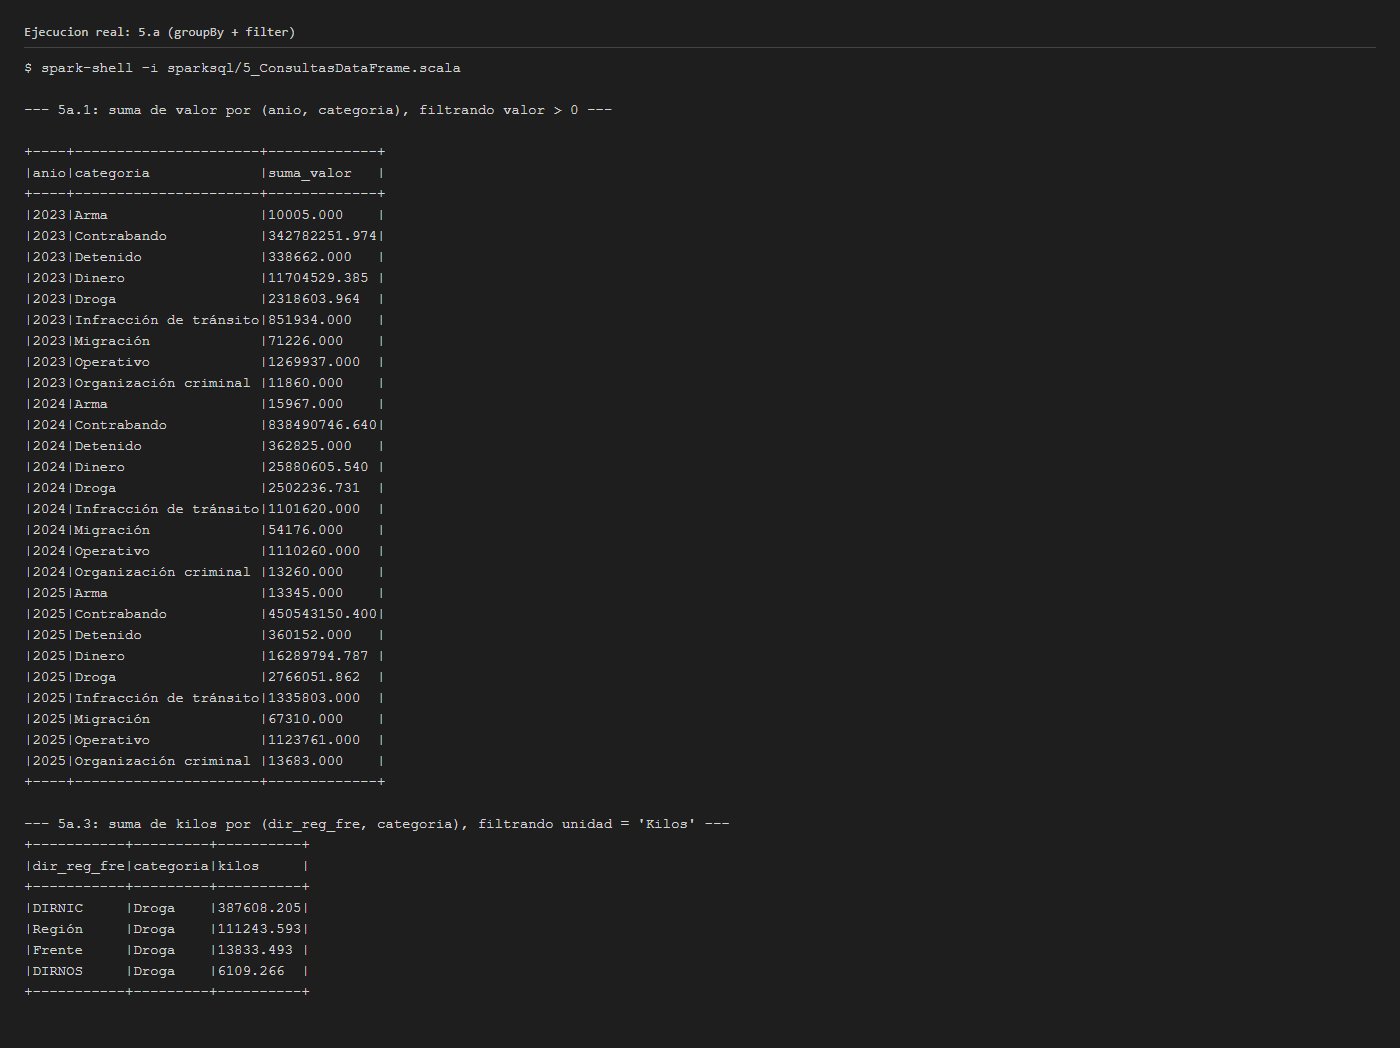
\includegraphics[width=0.95\linewidth]{capturas/img_5a.png}
\caption{Ejecuci\'on real de 5.a.1 y 5.a.3 en \texttt{spark-shell}.}
\end{figure}

\textbf{Interpretaci\'on.} La categor\'ia \texttt{Contrabando} domina en magnitud monetaria sobre
cualquier otra, porque valoriza mercader\'ia incautada completa (no solo dinero en efectivo); separarla
del resto evita que distorsione los promedios de las dem\'as categor\'ias.

\subsection{5.b -- Promedio de una columna y \texttt{orderBy} descendente}
\textbf{Promedio por categor\'ia:} \texttt{Operativo} 2070.90, \texttt{Dinero} 31\,840.98,
\texttt{Contrabando} 964\,430.35 (soles, promedio por registro).

\textbf{Dependencias ordenadas por suma total de \texttt{valor} (desc):} DIRPOFIS
(S/\,629\,764\,354.07), RP Puno (S/\,625\,303\,995.96), RP Tacna (S/\,107\,962\,632.05), DIVIAC
(S/\,72\,921\,809.11).
\begin{lstlisting}
val q5b2 = detalleDF.groupBy("dependencia").agg(sum("valor").as("total_valor")).orderBy(desc("total_valor"))
\end{lstlisting}
\begin{figure}[H]
\centering
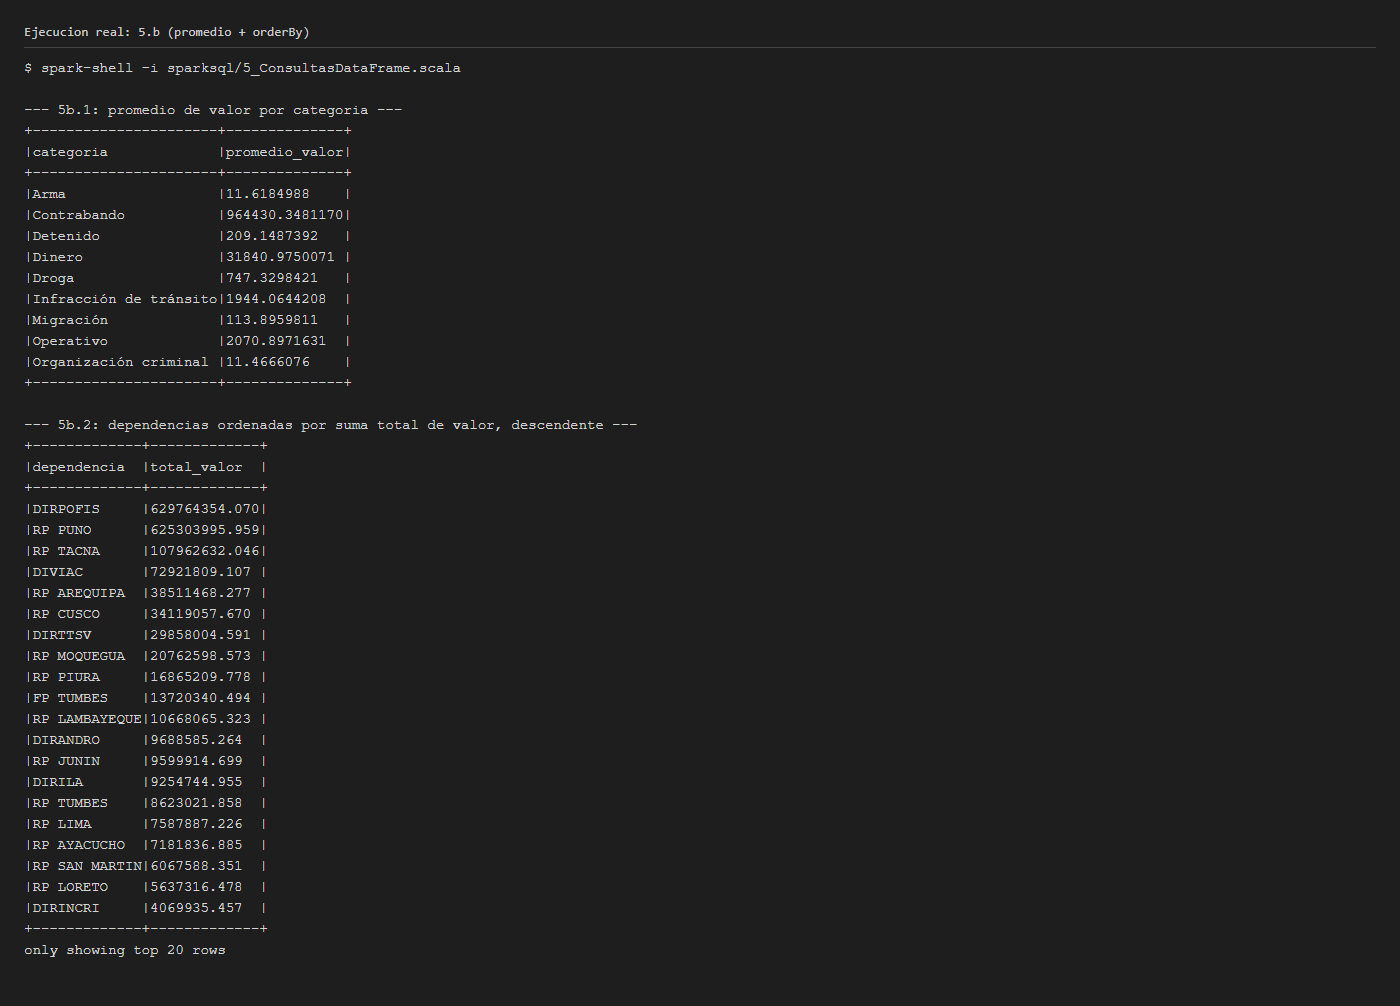
\includegraphics[width=0.95\linewidth]{capturas/img_5b.png}
\caption{Ejecuci\'on real de 5.b.1 y 5.b.2 en \texttt{spark-shell}.}
\end{figure}

\textbf{Interpretaci\'on.} Las sumas m\'as altas corresponden a dependencias con grandes decomisos de
\texttt{Contrabando (VALORIZACION)}, campo que domina en magnitud por estar expresado en soles de
mercader\'ia, no en unidades f\'isicas --confirma el mismo efecto visto en 5.a.1.

\subsection{5.c -- Cuatro \texttt{join}, uno de cada tipo}
\begin{table}[H]
\centering\small
\begin{tabular}{@{}llr@{}}
\toprule
\textbf{Tipo} & \textbf{Consulta} & \textbf{Filas resultantes}\\
\midrule
\texttt{inner} & hecho $\bowtie$ dim\_variable & 30\,456\\
\texttt{left\_outer} & dim\_dependencia $\bowtie$ hecho & 30\,456 (0 dependencias sin registros)\\
\texttt{right\_outer} & hecho $\bowtie$ dim\_dependencia & 30\,456\\
\texttt{full\_outer} & dim\_variable $\bowtie$ hecho & 30\,456 (0 variables sin uso)\\
\bottomrule
\end{tabular}
\caption{Los 4 tipos de join sobre hecho\_resultado\_operativo y sus dimensiones.}
\end{table}
\begin{figure}[H]
\centering
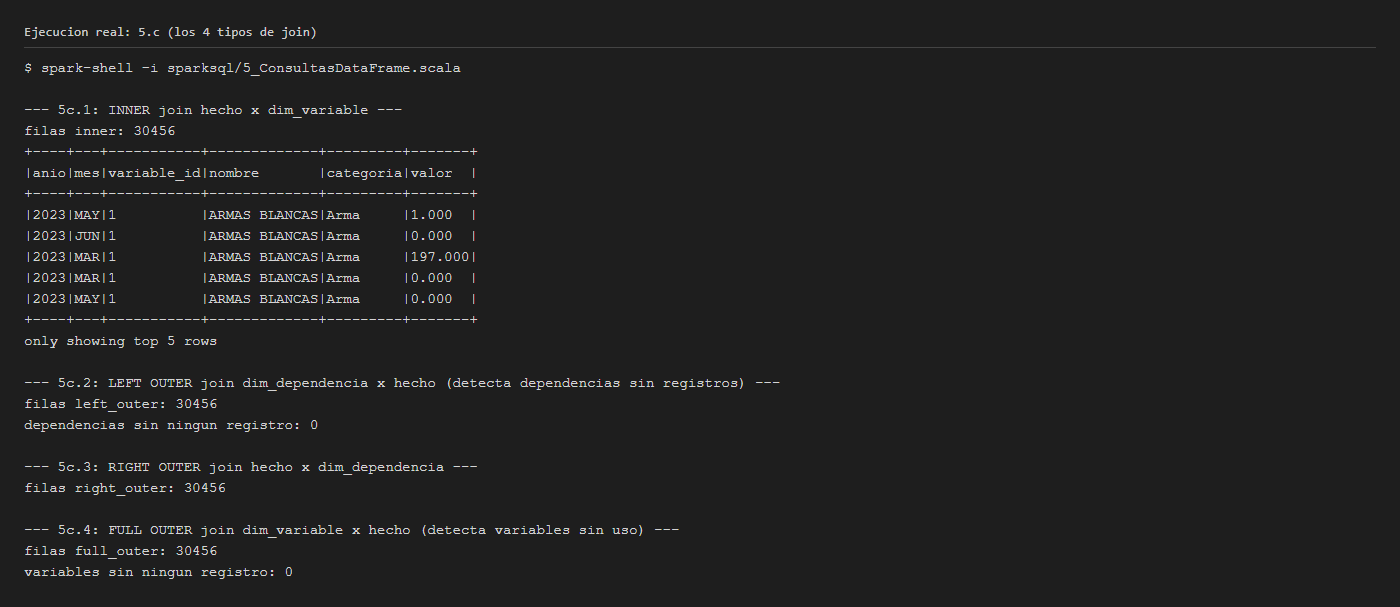
\includegraphics[width=0.85\linewidth]{capturas/img_5c.png}
\caption{Ejecuci\'on real de los 4 tipos de \texttt{join} de 5.c en \texttt{spark-shell}.}
\end{figure}

\textbf{Interpretaci\'on.} Que los 4 joins devuelvan exactamente 30\,456 filas, y que los
\texttt{LEFT}/\texttt{FULL} no encuentren dependencias ni variables ``hu\'erfanas'', confirma que la
integridad referencial del ETL (secci\'on~\ref{sec:etl}) es correcta: toda dependencia y toda variable de
las dimensiones tiene al menos un hecho asociado, y todo hecho referencia una dependencia y una variable
v\'alidas.

\subsection{5.d -- Cuatro consultas con \texttt{org.apache.spark.sql.functions.\_}}
\begin{enumerate}
  \item \texttt{round(avg(valor), 2)} por categor\'ia.
  \item Clasificaci\'on de \texttt{valor} en rangos con \texttt{when/otherwise}: 12\,137 registros ``sin
    incidencia'' (valor = 0), 10\,520 ``bajo'' ($<100$), 6587 ``medio'' ($<10\,000$), 1212 ``alto''.
  \item Etiqueta \texttt{concat\_ws(" - ", dependencia, mes, anio)} para identificar cada registro en un
    solo campo legible.
  \item \texttt{stddev(valor)} por categor\'ia: \texttt{Contrabando} tiene la mayor dispersi\'on
    ($1.30\times10^7$), \texttt{Arma} la menor (53.6).
\end{enumerate}
\begin{lstlisting}
val q5d2 = detalleDF.withColumn("rango_valor",
  when($"valor"===0,"sin incidencia").when($"valor"<100,"bajo")
  .when($"valor"<10000,"medio").otherwise("alto"))
\end{lstlisting}
\begin{figure}[H]
\centering
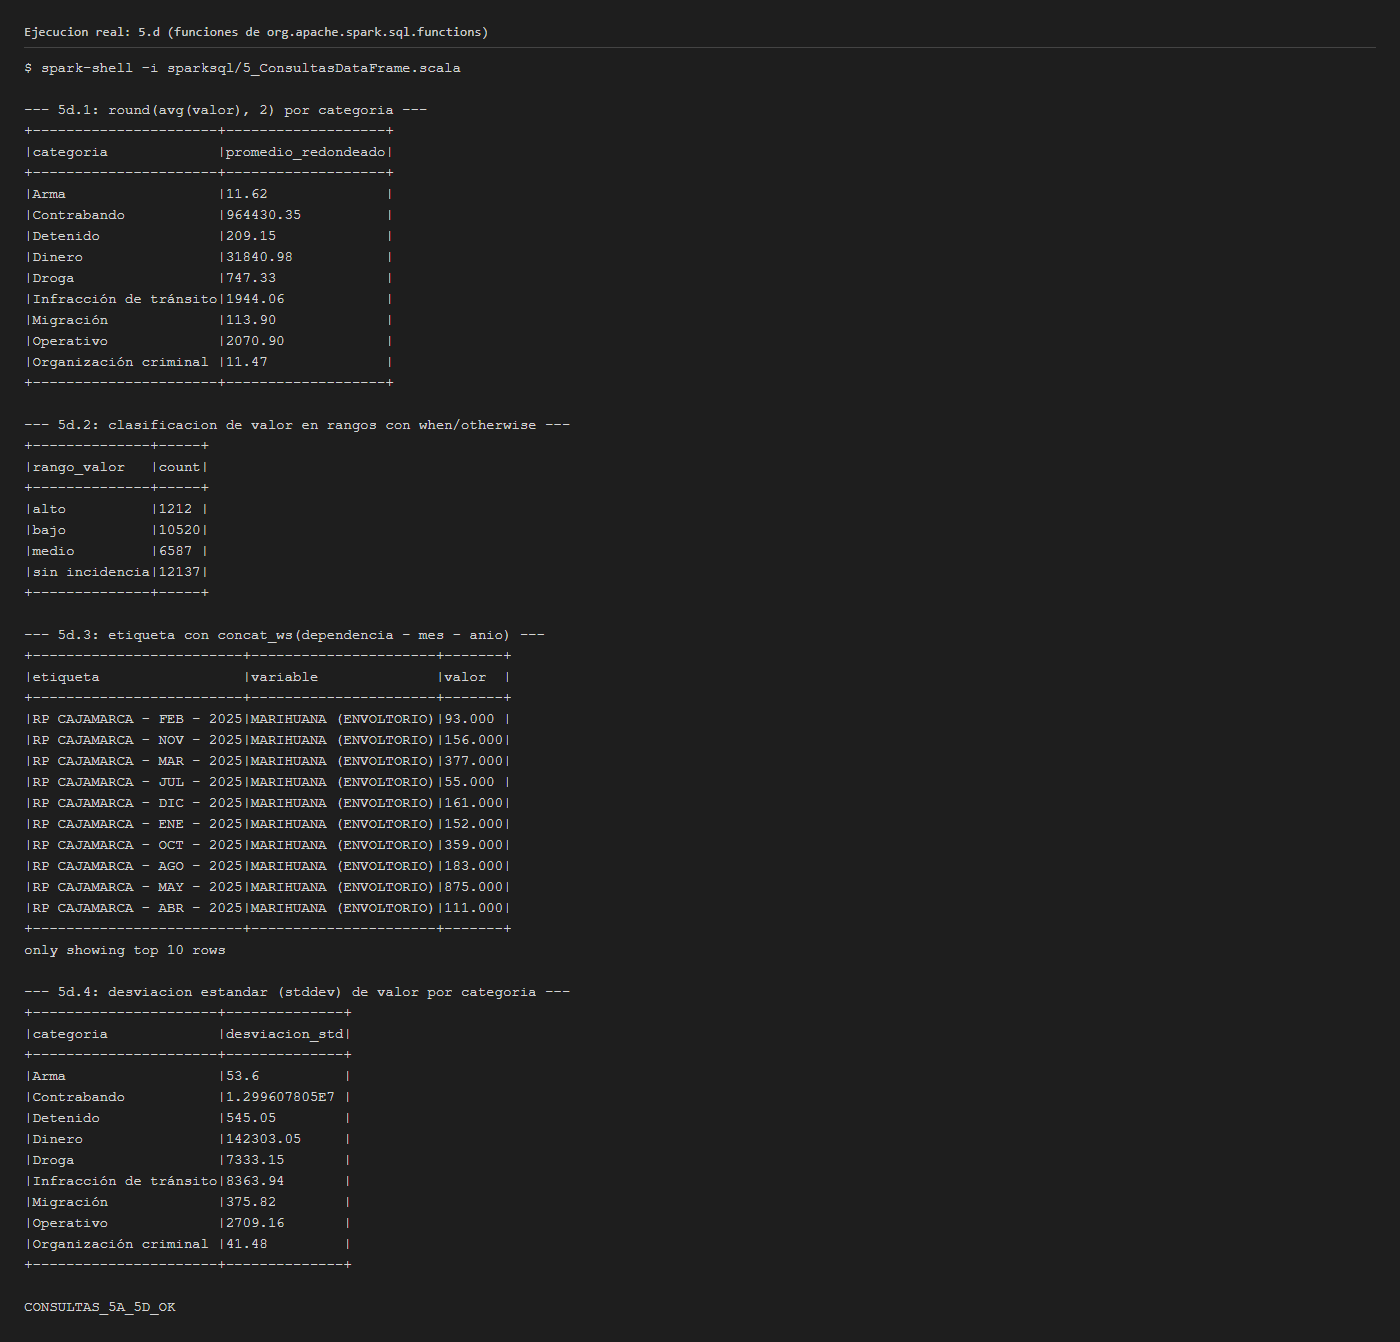
\includegraphics[width=0.95\linewidth]{capturas/img_5d.png}
\caption{Ejecuci\'on real de las 4 consultas de 5.d en \texttt{spark-shell}.}
\end{figure}

\textbf{Interpretaci\'on.} Que el 40\,\% de los registros (12\,137 de 30\,456) sea ``sin incidencia''
confirma algo esperable en datos de seguridad desagregados a nivel mensual y por dependencia: la mayor\'ia
de las combinaciones (dependencia, mes, tipo de resultado) no tiene actividad ese mes espec\'ifico, y el
an\'alisis agregado (sumas, promedios nacionales) es el que revela los patrones reales.

\section{Resultados: vistas temporales, Spark SQL puro y Excel}

\subsection{5.e -- Tres consultas con \texttt{JOIN} sobre vistas temporales}
Objetivos distintos a los de 5.c (que verificaban integridad referencial); aqu\'i se responde preguntas
de negocio concretas:
\begin{enumerate}
  \item \texttt{INNER JOIN} hecho+variable+dependencia, filtrando \texttt{categoria = 'Dinero'}, agrupado
    por dependencia y a\~no: ¿qu\'e dependencia incaut\'o m\'as dinero en qu\'e a\~no?
  \item \texttt{LEFT JOIN} dependencia+hecho+variable: total de \texttt{OPERATIVOS} por dependencia,
    incluyendo (con \texttt{COALESCE}) las que tuvieran cero.
  \item \texttt{FULL JOIN} variable+hecho filtrado a 2025: ¿qu\'e variables no tuvieron ning\'un registro
    en 2025? (ninguna; las 18 tienen al menos un registro ese a\~no).
\end{enumerate}
\begin{lstlisting}
val q5e1 = spark.sql("""
  SELECT d.nombre AS dependencia, h.anio, SUM(h.valor) AS dinero_incautado
  FROM hecho h
  INNER JOIN variable v ON h.variable_id = v.variable_id
  INNER JOIN dependencia d ON h.dependencia_id = d.dependencia_id
  WHERE v.categoria = 'Dinero'
  GROUP BY d.nombre, h.anio ORDER BY dinero_incautado DESC
""")
\end{lstlisting}

\begin{figure}[H]
\centering
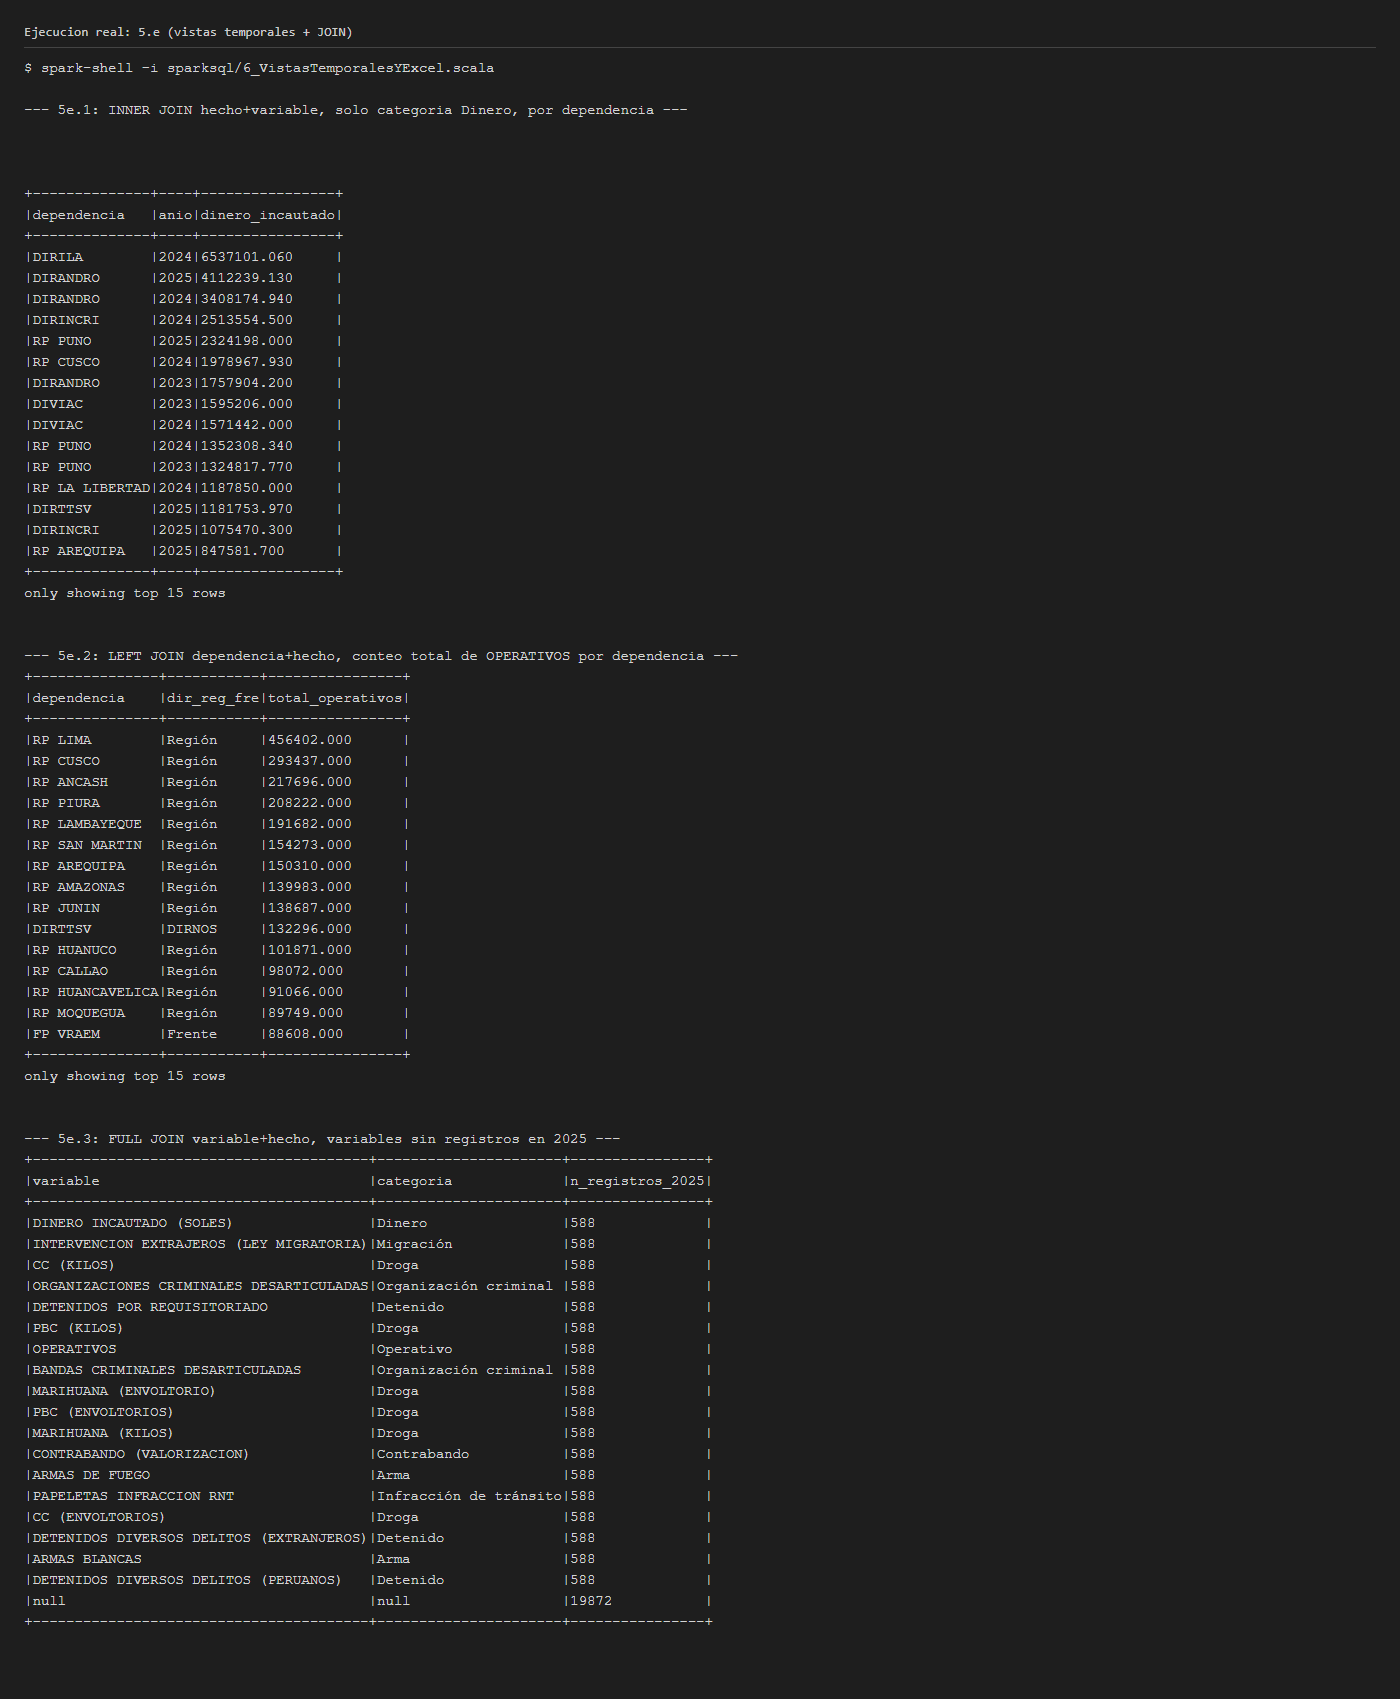
\includegraphics[width=0.75\linewidth]{capturas/img_5e.png}
\caption{Ejecuci\'on real de las 3 consultas de 5.e sobre vistas temporales.}
\end{figure}

\subsection{5.f -- Tres \texttt{ORDER BY} combinados con filtros}
\begin{enumerate}
  \item Registros de categor\'ia \texttt{Arma}, de mayor a menor valor (\texttt{LIMIT 10}).
  \item Registros de 2025 en dependencias clasificadas como \texttt{Regi\'on} (no Frente/DIRNIC/DIRNOS),
    de mayor a menor.
  \item Registros de \texttt{DINERO INCAUTADO} mayores a cero, de menor a mayor (para ver los decomisos
    m\'as peque\~nos que s\'i tuvieron actividad).
\end{enumerate}

\begin{figure}[H]
\centering
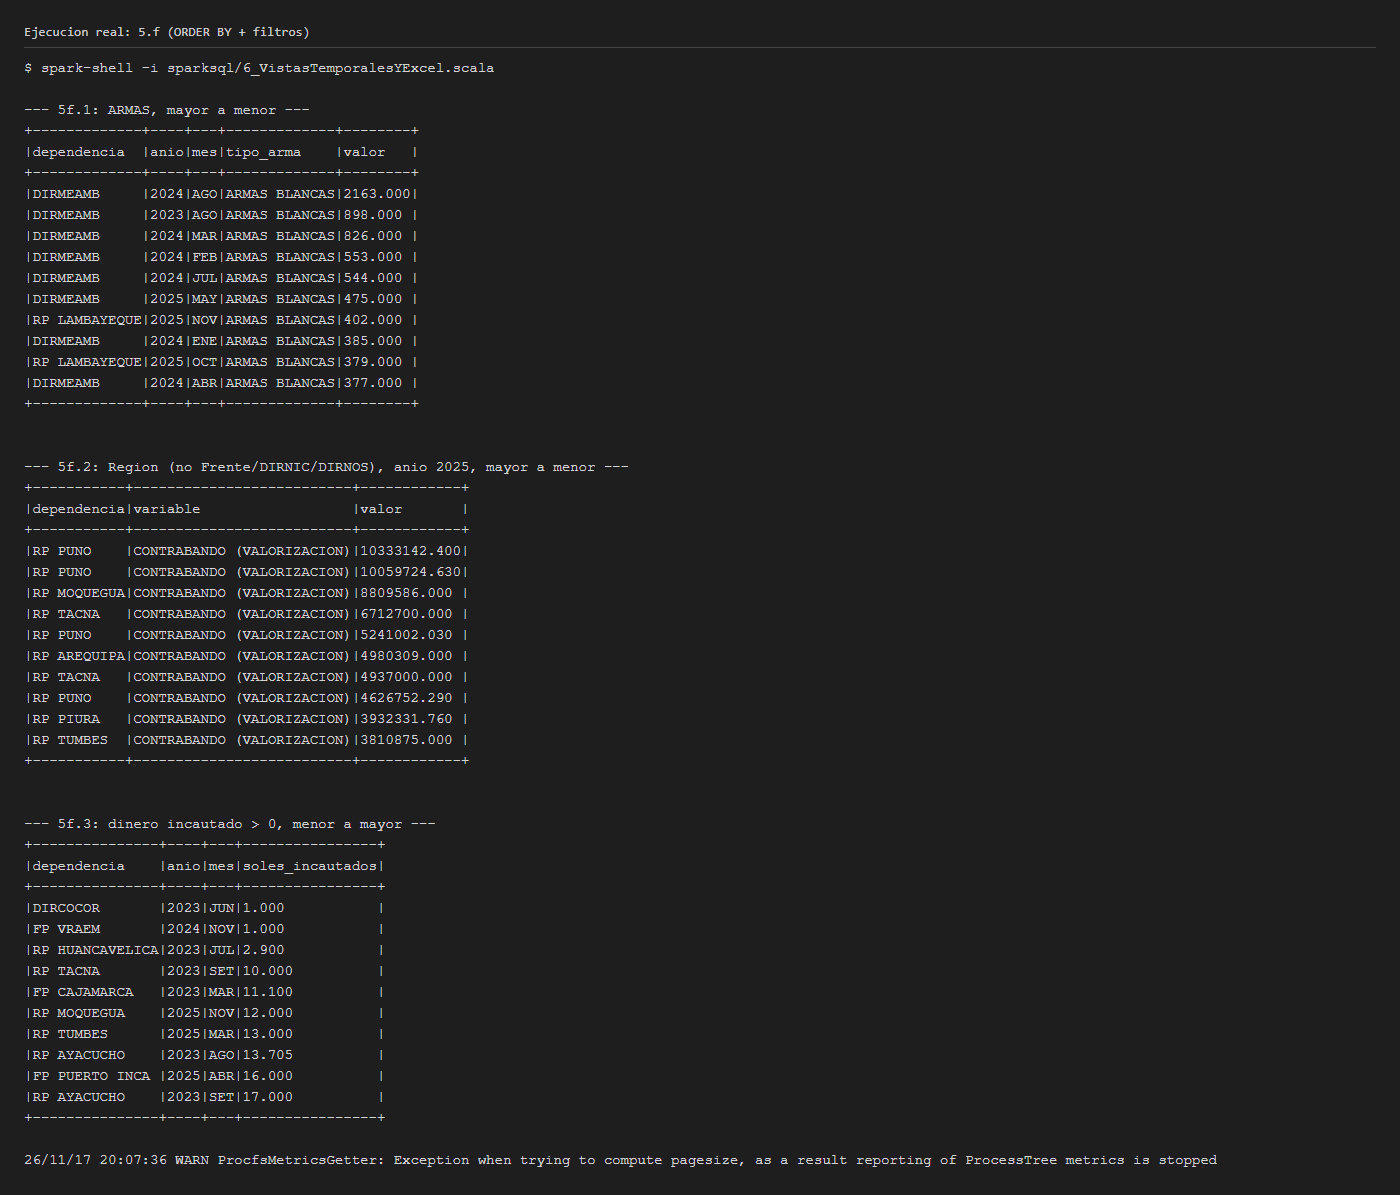
\includegraphics[width=0.85\linewidth]{capturas/img_5f.png}
\caption{Ejecuci\'on real de las 3 consultas de 5.f.}
\end{figure}

\subsection{5.g -- Exportaci\'on a Excel con Spark}
Los resultados de 5.e y 5.f se guardaron con la librer\'ia \texttt{spark-excel}
(\texttt{com.crealytics:spark-excel\_2.12:3.3.2\_0.19.0}, versi\'on compatible con Spark 3.3.2), una hoja
por consulta dentro de dos archivos (\texttt{PC3\_resultados\_5e.xlsx} con 3 hojas,
\texttt{PC3\_resultados\_5f.xlsx} con 3 hojas), usando \texttt{mode("overwrite")} para la primera hoja de
cada archivo y \texttt{mode("append")} para las siguientes (que en \texttt{spark-excel} agrega una hoja
nueva al mismo libro en vez de sobrescribirlo).
\begin{lstlisting}
df.coalesce(1).write.format("com.crealytics.spark.excel")
  .option("header","true").option("dataAddress", s"'$hoja'!A1")
  .mode(if (primera) "overwrite" else "append").save(ruta)
\end{lstlisting}

\begin{figure}[H]
\centering
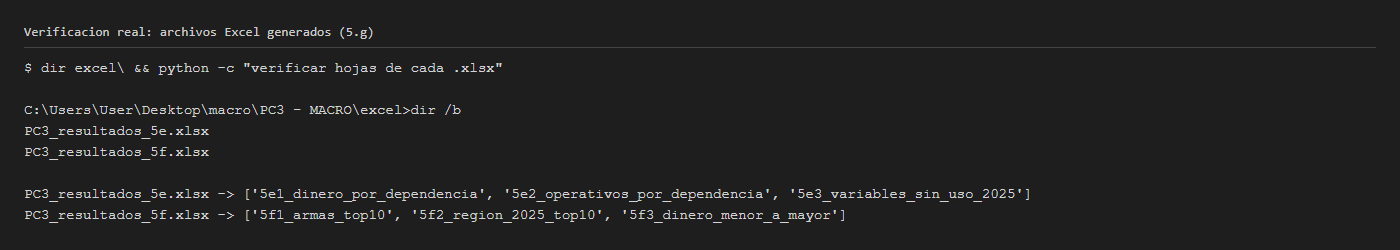
\includegraphics[width=0.85\linewidth]{capturas/img_excel.png}
\caption{Verificaci\'on real de los 2 archivos Excel generados y las 3 hojas de cada uno.}
\end{figure}

\section{Conclusiones}
\begin{enumerate}
  \item Se resolvieron 5 consultas en Scala sobre RDD con MapReduce puro (una de agrupamiento con
    m\'aximos/m\'inimos, una de estad\'isticos, y tres con MapReduce triple), 18 consultas con la API de
    DataFrame y vistas temporales de Spark SQL, y se export\'o un subconjunto a Excel, todo sobre el
    dataset de operaciones policiales del MININTER (30\,456 registros, 2023-2025).
  \item Se dise\~n\'o y pobl\'o un esquema en estrella en PostgreSQL mediante un proceso ETL completo
    (Extract-Transform-Load) programado \'integramente en Scala/Spark, incluyendo la correcci\'on de un
    problema real de calidad de datos (432 filas con regi\'on mal copiada).
  \item Los resultados se verificaron cruzando consultas independientes entre s\'i (el m\'aximo de dinero
    incautado coincide exactamente entre 3.a y 3.b) y comprobando la integridad referencial del esquema
    (los 4 tipos de \texttt{join} de 5.c no encuentran registros hu\'erfanos en ninguna direcci\'on).
  \item El hallazgo m\'as relevante: el dinero incautado promedio mensual m\'as que se duplic\'o de 2023 a
    2024 ($+121\%$) y luego cay\'o un tercio hacia 2025 ($-37\%$), consistente con la alta dispersi\'on
    (desviaci\'on est\'andar 4.5 veces el promedio) encontrada en esa misma variable.
  \item Todo el entorno (Spark, Scala, PostgreSQL) se instal\'o sin privilegios de administrador,
    usando las versiones port\'atiles/por usuario de cada herramienta.
\end{enumerate}

\end{document}
